%        File: pyne_ans.tex 
%     Created: 6.28.2012 

\documentclass{anstrans}
%%%%%%%%%%%%%%%%%%%%%%%%%%%%%%%%%%%
\title{PyNE : Python For Nuclear Engineering}
\author{Anthony~M.~Scopatz$^1$, Paul~K.~Romano$^2$, Paul~P.H.~Wilson$^3$, Kathryn~D.~Huff$^3$}

%% uncomment these next five only if using anstrans
\institute{$^1$ University of Chicago, $^2$ Massachusetts Institute of Technology, $^3$ University of Wisconsin }
\email{pyne-dev@googlegroups.com}
\usepackage{graphicx}
\usepackage{booktabs} % nice rules for tables
\usepackage{microtype} % if using PDF
\newcommand{\units}[1] {\:\text{#1}}%
\newcommand{\SN}{S$_N$}%{S$_\text{N}$}%{$S_N$}%

\date{}
%%%%%%%%%%%%%%%%%%%%%%%%%%%%%%%%%%%
\begin{document}
%%%%%%%%%%%%%%%%%%%%%%%%%%%%%%%%%%%%%%%%%%%%%%%%%%%%%%%%%%%%%%%%%%%%%%%%%%%%%%%%
\section{Introduction}

PyNE, or `Python for Nuclear Engineering'\footnote{http://pyne.github.com}, is a
nascent free and open source C++/Cython/Python package for performing common
nuclear engineering tasks.  This is intended as a base level tool kit - akin to
SciPy or Biopython - for common algorithms in the nuclear science and
engineering domain.

\section{Background}

While PyNE may be considered long overdue from an external perspective, the 
nuclear industry poses a uniquely high barrier to entry for free software.  
That closed source solutions are often easier to develop is an irony that 
increases the novelty of this package.

An initial hurdle for PyNE is the myriad of arcane file formats (both plain text
and binary) which have been industry standard since the 1960s.  Though obtuse 
specifications are not solely a nuclear problem, the scale of the number of formats 
is much greater.  Partly to blame is that some of these formats were enshrined 
in international law at a time when Fortran 2 was the language of choice.

Thus the emerging value of PyNE is that it allows new users to shortcut the tedious and 
error prone process of writing their own tools to parse these data and output file 
formats.  The current unfortunate state of affairs is due in part to huge institutional 
inertia on the part of the maintainers of such formats.  This manifests as a reluctance to 
develop or refactor new and existing codes in a modern open source manner.  PyNE seeks to 
increase human efficiency via a shared set of solutions rather than having every developer 
around the world replicate the same parsing routines.

Another major challenge for the community of PyNE developers is maintaining
the BSD license while explicitly avoiding any code which may be subject to 
export control.  Many nuclear engineering codes are open source in the sense
that the source code is distributed to developers who are then free to modify it.
However, due to the fear of illicit use for the development of weapons, these
same codes are then heavily export controlled and redistribution in any form is 
against their licenses and is often illegal.

Redistribution concerns are not limited to source code.  Basic nuclear data, 
while fundamentally un-copywritable under Western jurisprudence, may also 
be considered sensitive and subject to export control laws.  PyNE has developed
a three-tiered strategy to alleviate the data burden of the individual user based 
on the level of openness of the data. 

In spite of the above administrative concerns, PyNE's place in the nuclear software 
ecosystem requires that it have a general architecture.  Large portions of the code 
base are written in pure C or C++ and are built as Python-independent shared libraries. 
This enables other, compiled nuclear engineering codes to leverage PyNE.  Hence, the 
Cython layer has wrappers for C++ standard library containers (maps, 
sets, lists, etc) which implement the Python collections interface of the 
appropriate type.  Because of the high degree of factorization in PyNE, these wrappers 
could easily be reused by other projects.

%%%%%%%%%%%%%%%%%%%%%%%%%%%%%%%%%%%%%%%%%%%%%%%%%%%%%%%%%%%%%%%%%%%%%%%%%%%%%%%%

\section{Current Capabilities}

The following is an overview of the current capabilities of PyNE.
This covers briefly each major module and its relevance to nuclear 
engineering.  This is not meant to be a tutorial.  For such information
please refer to the PyNE user's guide \cite{PyNE:2012}.

\subsection{Nuclide Naming} 
There are a plethora of ways to represent nuclide names.  The 
\texttt{pyne.nucname} module may be used to convert between these various 
naming schemes. Currently the following naming conventions are supported: 
zzaaam, human readable names, MCNP, Serpent, NIST, and CINDER.  This module 
may convert between any of them.  Furthermore, it is implemented in C.


\subsection{Basic Nuclear Data}
The \texttt{pyne.data} module aims to provide quick access to very high fidelity 
nuclear data. Usually values are taken from the \texttt{nuc\_data.h5} library. 
This library is 
generated by the new \texttt{nuc\_data\_make} utility at install time.  Current 
data includes atomic masses, 
decay data, neutron scattering lengths, and simple cross section data. 63-group
neutron cross sections, photon cross sections, and fission product yields are
also added when CINDER is available on the machine of the user.  This module is 
implemented in C++.


\subsection{The Material Class} 
Materials are the primary container for radionuclides throughout PyNE. They map 
nuclides to mass weights, though they also contain methods for converting to and from 
atom fractions.  In many ways this class takes inspiration from numpy arrays 
and python dictionaries.  Materials are implemented in C++ and support both text
and HDF5 persistence.  This class may be found within \texttt{pyne.material}.


\subsection{CCCC Formats}
The \texttt{pyne.cccc} module contains a number of classes for reading various cross section, 
flux, geometry, and data files with specifications given by the Committee for 
Computer Code Coordination. The following types of files can be read using 
classes from this module: ISOTXS, DLAYXS, BRKOXS, RTFLUX, ATFLUX, RZFLUX, MATXS, 
and SPECTR.

\subsection{ACE Module}

One of the most common data formats used to represent pointwise
linearly-interpolatable cross sections is the ACE (A Compact ENDF) format. This
format was introduced by LANL for use in the MCNP \cite{mcnp} code and is now
used by the Serpent \cite{serpent} and OpenMC \cite{openmc} Monte Carlo codes as
well. While there are a variety of resources that allow a user to inspect and
plot data directly from ENDF, there has generally been no good means of looking
at processed data in the ACE format that is actually used in Monte Carlo
simulations. As such, a module has been added to PyNE to parse and store data
from ASCII or binary ACE files. A front-end graphical user interface is also in
development that will give the user an easy interface to view and compare both
cross sections and secondary energy and angle
distributions. Figure~\ref{fig:ace-gui} shows cross section data for Pu-239
being plotted within the GUI.
\begin{figure}[ht]
  \centering
  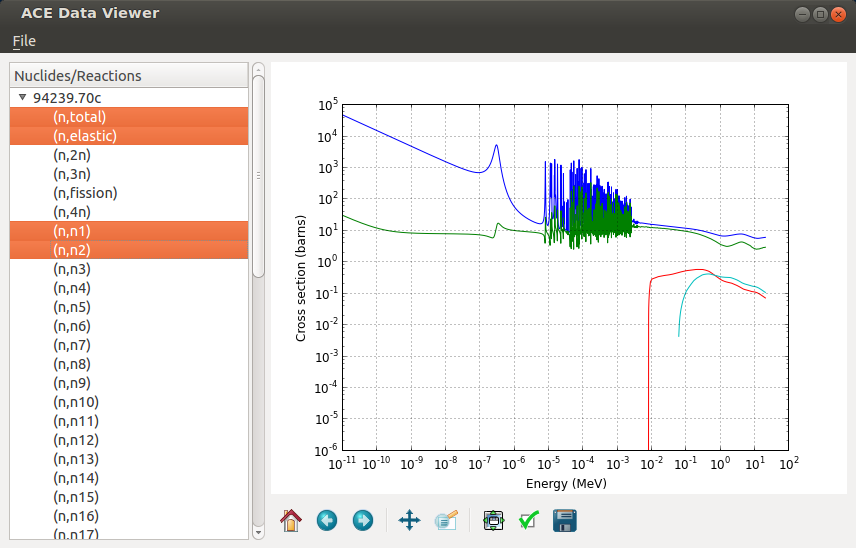
\includegraphics[width=3.3in]{ace-gui.png}
  \caption{Front-end graphical user interface for plotting ACE format data in
    PyNE.}
  \label{fig:ace-gui}
\end{figure}


\subsection{Cross Section Interface} 
The \texttt{pyne.xs} sub-package provides a top-level interface for computing 
(and caching) multigroup neutron cross sections. These cross sections will be 
computed from a variety of available data sources.  Nominally these are stored 
in the \texttt{nuc\_data.h5} HDF5 library which was generated by \texttt{nuc\_data\_make}
at installation time.  The library is searched for the following data sets in the 
following order of preference: 

\begin{enumerate}
    \item CINDER 63-group cross sections \cite{cinder},
    \item A two-point fast/thermal interpolation (using `simple\_xs' data from KAERI \cite{kaeri}),
    \item or physical models implemented in this sub-package.
\end{enumerate}

In the future, this package will support generating multigroup cross sections 
from user-specified pointwise data sources (such as ENDF or ACE files).  In future 
versions of PyNE, this 
package may also include SCALE multigroup cross sections, if available \cite{scale}.


\subsection{ORIGEN 2.2 Support}
The \texttt{pyne.origen22} module provides an interface for reading, writing, and 
merging certain ORIGEN 2.2 \cite{origen} input and output files.  Specifically, 
tapes 4, 5, 6, and 9 are currently supported.  Other decks could be supported in 
the future with relative ease if the need or interest arises.


\subsection{Serpent Support} 
Serpent \cite{serpent} is a continuous energy Monte Carlo reactor physics code.  
Pyne contains support for reading in Serpent's three types of output files: 
\texttt{*.res}, \texttt{*.dep}, and \texttt{*.det}.  These are all in Matlab 
\texttt{*.m} format and are read in 
as Python dictionaries of numpy arrays and Materials.  They may be optionally 
written out to corresponding \texttt{*.py} files and imported later.

\subsection{NJOY Module}
Recently the developers of PyNjoy \cite{dragon}, a set of Python bindings for processing
nuclear data using NJOY, agreed to have their work integrated with the PyNE
project as a new NJOY module. This will help to encourage active development and
wider participation in the project.

The NJOY module provides a simple method of generating nuclear data in a variety
of formats from raw ENDF data without the user having to worry about the exact
format of the NJOY input files. Thus, with a single Python script, it is
possible to process thousands of nuclides at once rather than managing
many NJOY input files.


%%%%%%%%%%%%%%%%%%%%%%%%%%%%%%%%%%%%%%%%%%%%%%%%%%%%%%%%%%%%%%%%%%%%%%%%%%%%%%%%
\section{Conclusions}
Over the past year, the PyNE development team has formed a community 
which has successfully overcome many initial hurdles.  In addition to
the regular burden of starting a new open source project, the nuclear 
domain contains special concerns about export control and non-proliferation.
By maintaining a conservative development strategy, only methods and data
which are truly open make it into the PyNE code base.  Even with these 
restraints the number of tools possible is very large.

With over 22000 lines of C++, Cython, and Python code, PyNE has just begun to
implement what is in its purview.  The more modules that PyNE has, the more
utilities may be composed using it.   Noting the possibility for 
`scope explosion,' the development team is committed to adhering to 
modern software quality development standards.  At a minimum, all contributions 
to PyNE must be tested, documented, and follow the official Python coding
standard.

Future work may include further NJOY-like capabilities, a fully-featured 
MCNP interface, a common nuclear materials database, various infinite medium
diffusion solvers, deep geologic repository modeling functionality, and Bateman 
equation solvers.

%%%%%\acknowledgements
\section*{Acknowledgements}
The authors would like to recognize additional code contributions by 
Christopher Dembia, Robert Flanagan, and Eric Relson.  Moreover, we 
would like to thank
Seth Johnson,
Joshua Peterson, 
Rachel Slaybaugh, 
Nick Touran,
and Morgan White
for their inspiration, guidance, and testing.


%%%%%%%%%%%%%%%%%%%%%%%%%%%%%%%%%%%%%%%%%%%%%%%%%%%%%%%%%%%%%%%%%%%%%%%%%%%%%%%%
\nocite{*}
\bibliographystyle{ans}
\bibliography{pyne_ans2012}
\end{document}


